
\todo{Create a Diagram and have my Question in the middle. From reading my first Journal paper, I'll add key branches to the diagram.}

\todo{In the diagram - Reader can identify - This is my Diagram - This is my Question and I have the relevant things properly cited and referenced. How to add citation to a diagram. }

\todo{So I'll talk about these themes from the Figure and how they are connected to my work. logically.Hence the Chapters bence said. This should be in the diagram.  }

\section{Data Science}

\begin{figure}[h!]
	\centering
	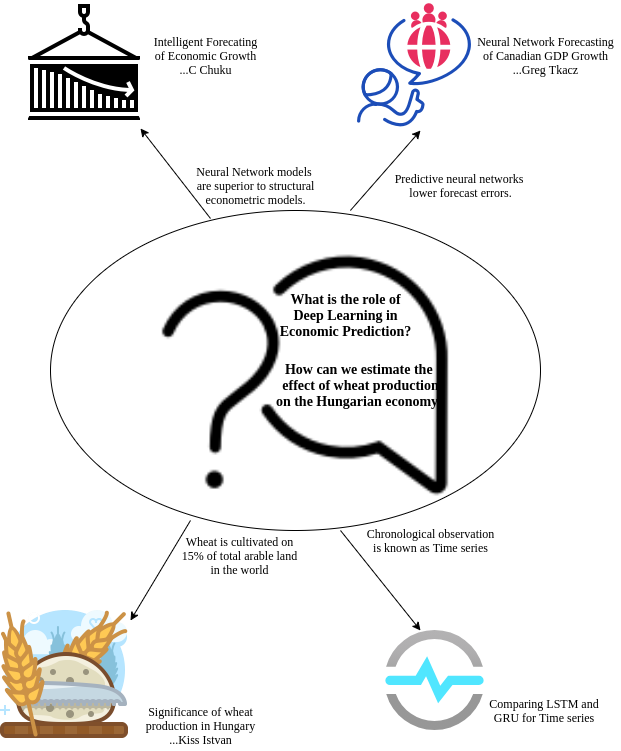
\includegraphics[width=0.75\textwidth, height=0.75\columnwidth]{Related_Works.png}
	\caption{Related Works.\protect\cite{tkacz2001neural, chuku2017intelligent, kiss2011significance, yamak2019comparison}}
	\label{fig:relatedWorks}
\end{figure}








Intelligence is the ability to process information to inform future decisions. The field of Artificial Intelligence is the field which focuses on building algorithm models (in this case, Artificial Intelligence \cite{black2009books} Algorithms) that can do this as well - that is - process information to inform future decisions.

Machine Learning itself is a subset of AI that focuses on teaching a machine how to do this without being explicitly programmed. 

Deep Learning is a subset of Machine Learning which takes this idea even further. It allows us to automatically extract the useful pieces of information needed to inform these future predictions.

Availability of localized and external data can help to practice *Precision Agriculture*

Like all other neural networks, deep-learning models don't take as input raw text:
they only work with numeric tensors. Vectorizing text is the process of transforming text
into numeric tensors. This can be done in multiple ways


Data Science encompasses making awesome visualizations and models using data. As a field of Computer Science, it has created as much positive impact in our society. Impact could be in the form of insights, in the form of data products or in the form of product recommendations for a company. In order to achieve these things, we need tools like writing code, machine learning models or data visualizations.


According to this article by Usama Fayyad \cite{fayyad1996data} data mining is referred to  as the overall process of discovering useful information from data. William S. Cleveland, \cite{cleveland2001data}   who at that time was a Distinguished Member of Technical Staff in the Statistics Research Department at Bell Labs, Murray Hill, defined data science as it is used today. He did that by combining computer science with data mining. He made statistics a lot more technical because he believed it would expand the possibilities of data mining and produce a powerful force for innovation. Now, we can take advantage of computational power for statistics.



\subsection{Technical Advancement}
Around this time, \textbf{web 2.0} emerged. Websites aren't simply digital pamphlets anymore, but a medium for shared experience among millions of users. These are websites like:
\begin{itemize}
	\item \textbf{MySpace:} 2003
	\item \textbf{Facebook:} 2004
	\item \textbf{YouTube:} 2005	
\end{itemize}

As users, we can now interact with these websites - post, comment, share - leaving our digital footprints on the Internet. That's a lot of data and soon enough, it became too much to handle using traditional technologies. This opened a world of possibilities in finding insights using data. So the rise in data sparked the rise of data science to support the needs of businesses to draw insights from their massive unstructured data sets. This abundance of data now makes it possible to train machines with a data-driven rather than a knowledge-driven approach. Deep learning is no longer an abstract academic concept in this thesis paper. It is a tangible useful class of machine learning model for agricultural data applications.

\section{Machine Learning Workflow}
From predicting economic growth to detecting cancers, Machine Learning has granted computer systems entirely new abilities. The first step to solving a Machine Learning task is to define the problem and assemble a data-set. The data-set has to be one with integrity. Choosing a measure of success and deciding on a validation protocol are the next logical steps. The most important step in building a Machine Learning model is the preparation of the data. It won't occur in a real-life situation that raw data is ready to be fed into a machine model. 

Once the data is ready, the model can be built. At first, we build one that over-fits. Afterwards this model is regularized and its hyper-parameters tuned. 

\begin{figure}[h!]
	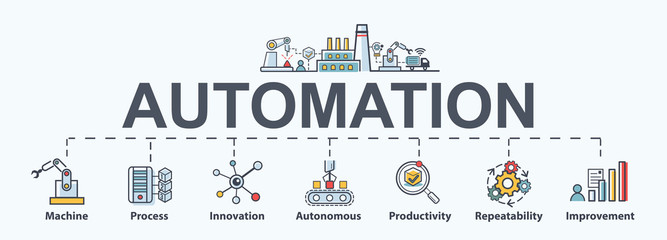
\includegraphics[width=\textwidth,height=\textheight,keepaspectratio]{workflow.png}
	\caption{Machine Learning Workflow.\protect\cite{division_2000, charfeddine2020reviewing, krose1993introduction}}
	\label{fig:workflow}
\end{figure}

Figure \ref{fig:workflow} shows the workflow of a typical Machine Learning model.
